All results in this section are for the \emph{test period}, water years
2017--2025, which no tuning or selection step has seen. It is run as three
3-year windows (WY2017--19, 2020--22, 2023--25), each started from the
observed Lake McClure storage on October~1 and with the same forecast
errors for every policy. The period is demanding: WY2017 and WY2023 are
the two wettest years of the record, and WY2020--2022 is a three-year
drought.

\subsection{Summary of the operating modes}

\begin{table}[h]
\centering\small
\setlength{\tabcolsep}{4pt}
\begin{tabular}{@{}lrrrrrrrrrr@{}}
\toprule
 & \multicolumn{2}{c}{Irrigation [\%]} & Flood & Energy & River & \multicolumn{4}{c}{Functional-flow score} & \\
\cmidrule(lr){2-3}\cmidrule(lr){7-10}
Policy & mean & worst yr & d/yr & GWh/yr & hm$^3$/yr & all & dry & mod. & wet & $J_{\mathrm{ff}}$\\
\midrule
MIF rule & 99.9 & 99.1 & 6.1 & 311 & 681 & 0.57 & 0.70 & 0.54 & 0.49 & -1.0 \\
Prescribed FF rule & 97.3 & 85.0 & 7.0 & 319 & 715 & 0.93 & 0.95 & 0.95 & 0.91 & 6.5 \\
Unimpaired flow (no dam) & -- & -- & -- & -- & -- & 0.88 & 0.88 & 0.92 & 0.87 & -- \\

\bottomrule
\end{tabular}
\caption{Test period WY2017--2025. Irrigation: delivered volume as \% of
demand, mean over the nine years and worst year. Flood: days with river
flow above $\Qsafe$. River: mean annual river flow below the dam (releases
plus spill). Functional-flow scores by the May~1 declared year type.
$J_{\mathrm{ff}}$: mean per-year reward under the Scenario~3 weights
(supply $+$ flood $+$ functional flows), the common yardstick. The last row
scores the unimpaired inflow itself, as if there were no dam.}
\label{tab:test}
\end{table}

Table~\ref{tab:test} and Figure~\ref{fig:tradeoff} summarize the
comparison. Read them as a trade-off between two goods: water delivered
to the canal, and how closely the river below the dam follows a
functional hydrograph.

\begin{itemize}
\item \textbf{Minimum instream flow (Scenario~1)} is almost free for
  irrigation: 99.9\% of demand is delivered, and even the worst drought
  year gets 99\%. Ecologically it is poor. The functional-flow score is
  0.57 against 0.88 for the unimpaired river, and lowest in wet years
  (0.49). The licence flows supply no fall pulse, no spring pulse and no
  managed recession. Most of the score the river does get comes from
  uncontrolled spill in wet years, which is not a managed outcome.
\item \textbf{Prescribed functional flows (Scenario~2)} lift the score to
  0.93, above the unimpaired river, because the schedule is built to meet
  the median-based targets every year. The cost is concentrated in the
  drought: overall delivery drops only to 97.3\%, but WY2022, the third dry
  year in a row, delivers 85\% of demand. The extra river water averages
  about 34~hm$^3$/yr, roughly 5\% of the irrigation demand, but it must
  be released in dry years too, when it hurts most.
\end{itemize}

\noindent Flood days (6--7 per year) are nearly the same for both: they come
from WY2017 and WY2023, when inflows far exceeded the safe channel capacity
whatever the operation. Energy differs little, since both outlets pass
the same powerhouse and the total release is set mostly by the demand.

\begin{figure}[h]
\centering
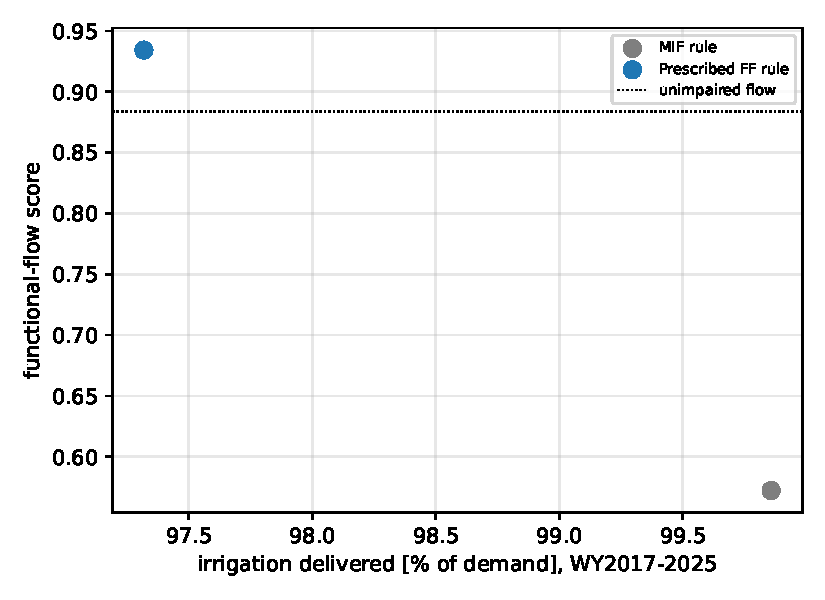
\includegraphics[width=0.6\textwidth]{figures/tradeoff.pdf}
\caption{Irrigation delivered vs functional-flow score, WY2017--2025. Up and
to the right is better. The dotted line is the score of the unimpaired
river.}
\label{fig:tradeoff}
\end{figure}

\subsection{Year by year}
Figure~\ref{fig:peryear} breaks the comparison down by water year. Two
patterns stand out. First, the functional-flow gain of the prescription is
largest in wet and moderate years (2017--2019, 2023--2025). In those years
the minimum-flow operation stores or diverts the spring snowmelt that a
functional hydrograph would pass downstream. Second, the irrigation cost
of the prescription appears only in WY2021 and WY2022, at the end of the
drought. By then storage has fallen to about 250~hm$^3$ under the
prescription, against about 330~hm$^3$ under minimum flows
(Figure~\ref{fig:hydro2020}), and the hedging rule cuts deliveries. This
is the classic problem with a static e-flow schedule. It spends water
early in a drought without knowing that the drought will last, and the
bill arrives two years later, in irrigation.

\begin{figure}[h]
\centering
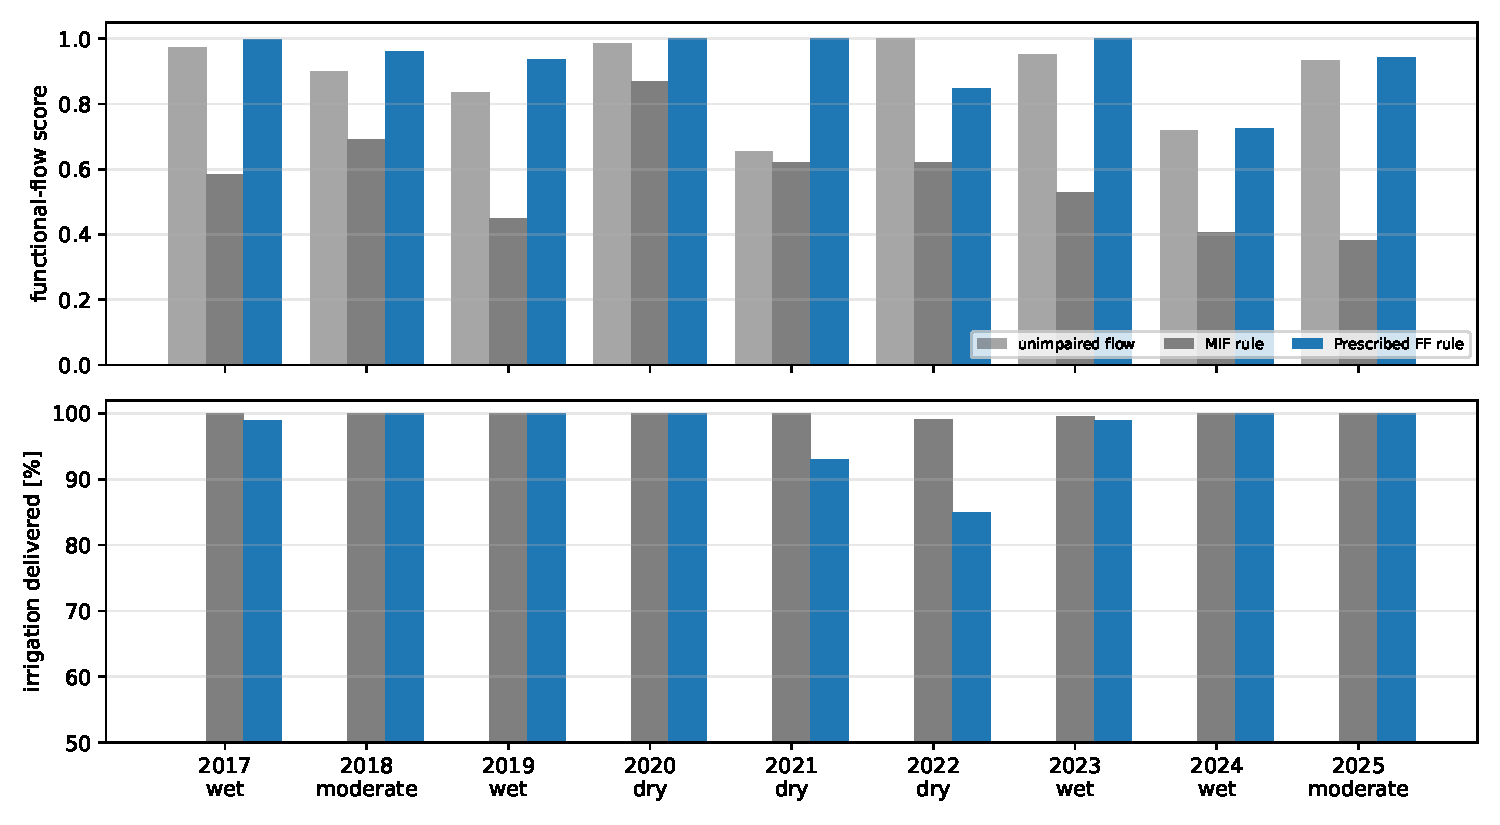
\includegraphics[width=\textwidth]{figures/per_year.pdf}
\caption{Functional-flow score (top) and irrigation delivered (bottom) by water
year, with the year type declared on May~1.}
\label{fig:peryear}
\end{figure}

\begin{table}[h]
\centering\footnotesize
\setlength{\tabcolsep}{3.5pt}
\begin{tabular}{@{}lllrrrrrrrr@{}}
\toprule
Policy & WY & type & Irr.\ [\%] & Flood d & FA & WB & PK & SP & DS & FF\\
\midrule
MIF rule & 2017 & wet & 100.0 & 17 & 0.00 & 0.74 & 1.00 & 0.99 & 0.19 & 0.58 \\
MIF rule & 2018 & moderate & 100.0 & 0 & 1.00 & 0.43 & 1.00 & 0.90 & 0.13 & 0.69 \\
MIF rule & 2019 & wet & 100.0 & 7 & 0.00 & 0.56 & 0.99 & 0.54 & 0.17 & 0.45 \\
MIF rule & 2020 & dry & 100.0 & 0 & 1.00 & 1.00 & -- & 0.48 & 1.00 & 0.87 \\
MIF rule & 2021 & dry & 100.0 & 0 & 0.00 & 1.00 & -- & 0.48 & 1.00 & 0.62 \\
MIF rule & 2022 & dry & 99.1 & 0 & 0.00 & 1.00 & -- & 0.48 & 1.00 & 0.62 \\
MIF rule & 2023 & wet & 99.6 & 31 & 0.00 & 0.28 & 1.00 & 0.99 & 0.37 & 0.53 \\
MIF rule & 2024 & wet & 100.0 & 0 & 1.00 & 0.45 & 0.00 & 0.44 & 0.13 & 0.41 \\
MIF rule & 2025 & moderate & 100.0 & 0 & 1.00 & 0.41 & 0.00 & 0.45 & 0.05 & 0.38 \\
\midrule
Prescribed FF rule & 2017 & wet & 99.0 & 23 & 1.00 & 1.00 & 1.00 & 0.98 & 1.00 & 1.00 \\
Prescribed FF rule & 2018 & moderate & 100.0 & 0 & 1.00 & 0.81 & 1.00 & 1.00 & 1.00 & 0.96 \\
Prescribed FF rule & 2019 & wet & 100.0 & 7 & 1.00 & 0.71 & 1.00 & 0.98 & 1.00 & 0.94 \\
Prescribed FF rule & 2020 & dry & 100.0 & 0 & 1.00 & 1.00 & -- & 1.00 & 1.00 & 1.00 \\
Prescribed FF rule & 2021 & dry & 93.0 & 0 & 1.00 & 1.00 & -- & 1.00 & 1.00 & 1.00 \\
Prescribed FF rule & 2022 & dry & 85.0 & 0 & 0.39 & 1.00 & -- & 1.00 & 1.00 & 0.85 \\
Prescribed FF rule & 2023 & wet & 98.9 & 33 & 1.00 & 1.00 & 1.00 & 1.00 & 1.00 & 1.00 \\
Prescribed FF rule & 2024 & wet & 100.0 & 0 & 1.00 & 0.48 & 0.14 & 1.00 & 1.00 & 0.72 \\
Prescribed FF rule & 2025 & moderate & 100.0 & 0 & 1.00 & 0.71 & 1.00 & 1.00 & 1.00 & 0.94 \\

\bottomrule
\end{tabular}
\caption{Component scores per water year (FA fall pulse, WB wet-season
baseflow, PK peak flow, SP spring pulse and recession, DS dry-season
baseflow; ``--'' where a component does not apply).}
\label{tab:years}
\end{table}

\noindent Table~\ref{tab:years} shows which components carry the
difference. Under minimum flows, the fall pulse (FA) and the spring
pulse and recession (SP) are mostly missing, and the dry-season baseflow
(DS) of wet years is far below what the natural river would carry. The
prescription meets almost everything. What it still misses comes from
deciding under forecast uncertainty: a wet-season baseflow or peak flow
sized for the year type declared in winter, in a year that the May~1
forecast then classes differently (Section~\ref{sec:yeartype}).

\subsection{Hydrographs}
Figures~\ref{fig:hydro2017}--\ref{fig:hydro2023} show what the operations
look like day by day: river flow against the unimpaired inflow (log
scale), storage, and canal delivery against demand.

\begin{figure}[p]
\centering
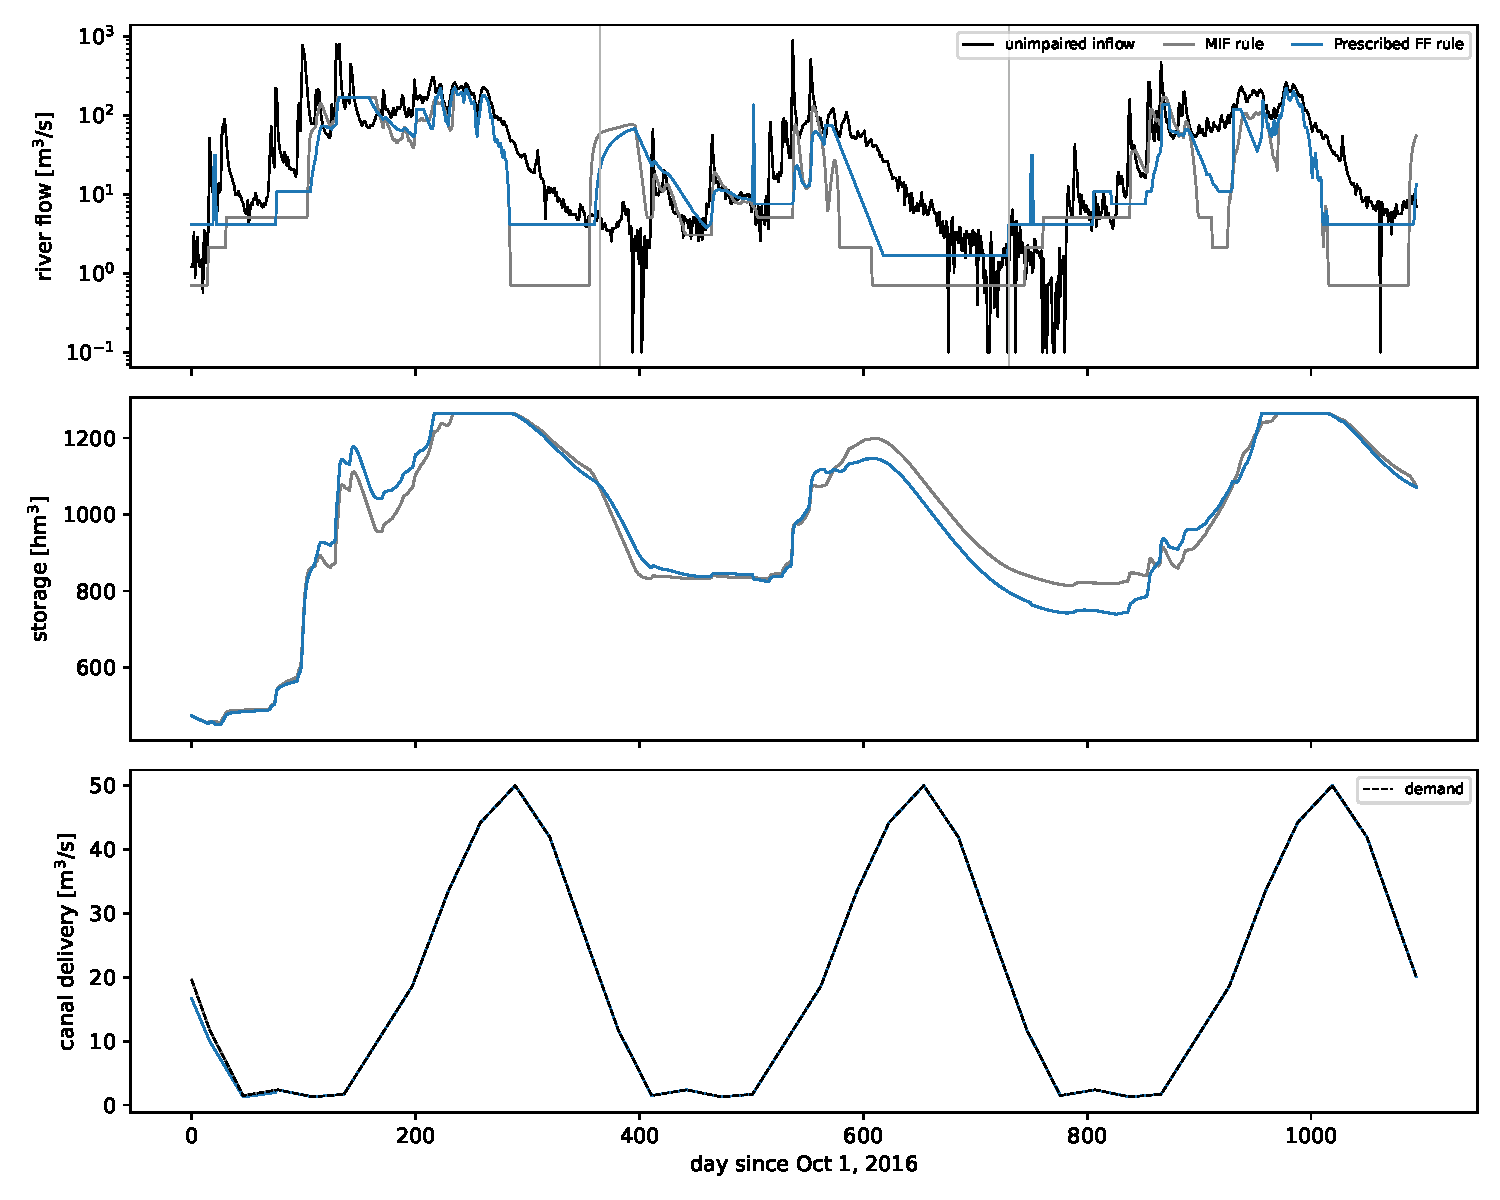
\includegraphics[width=0.92\textwidth]{figures/hydrograph_2017.pdf}
\caption{WY2017--2019 (wet, moderate, wet). The 2017 snowmelt fills the
reservoir under both operations and forces spill, i.e.\ flood flows that no
operation could avoid. Under the prescription the spring pulse and the
gradual recession are visible in every year. Under minimum flows the river
drops to the licence floor as soon as the spill ends.}
\label{fig:hydro2017}
\end{figure}

\begin{figure}[p]
\centering
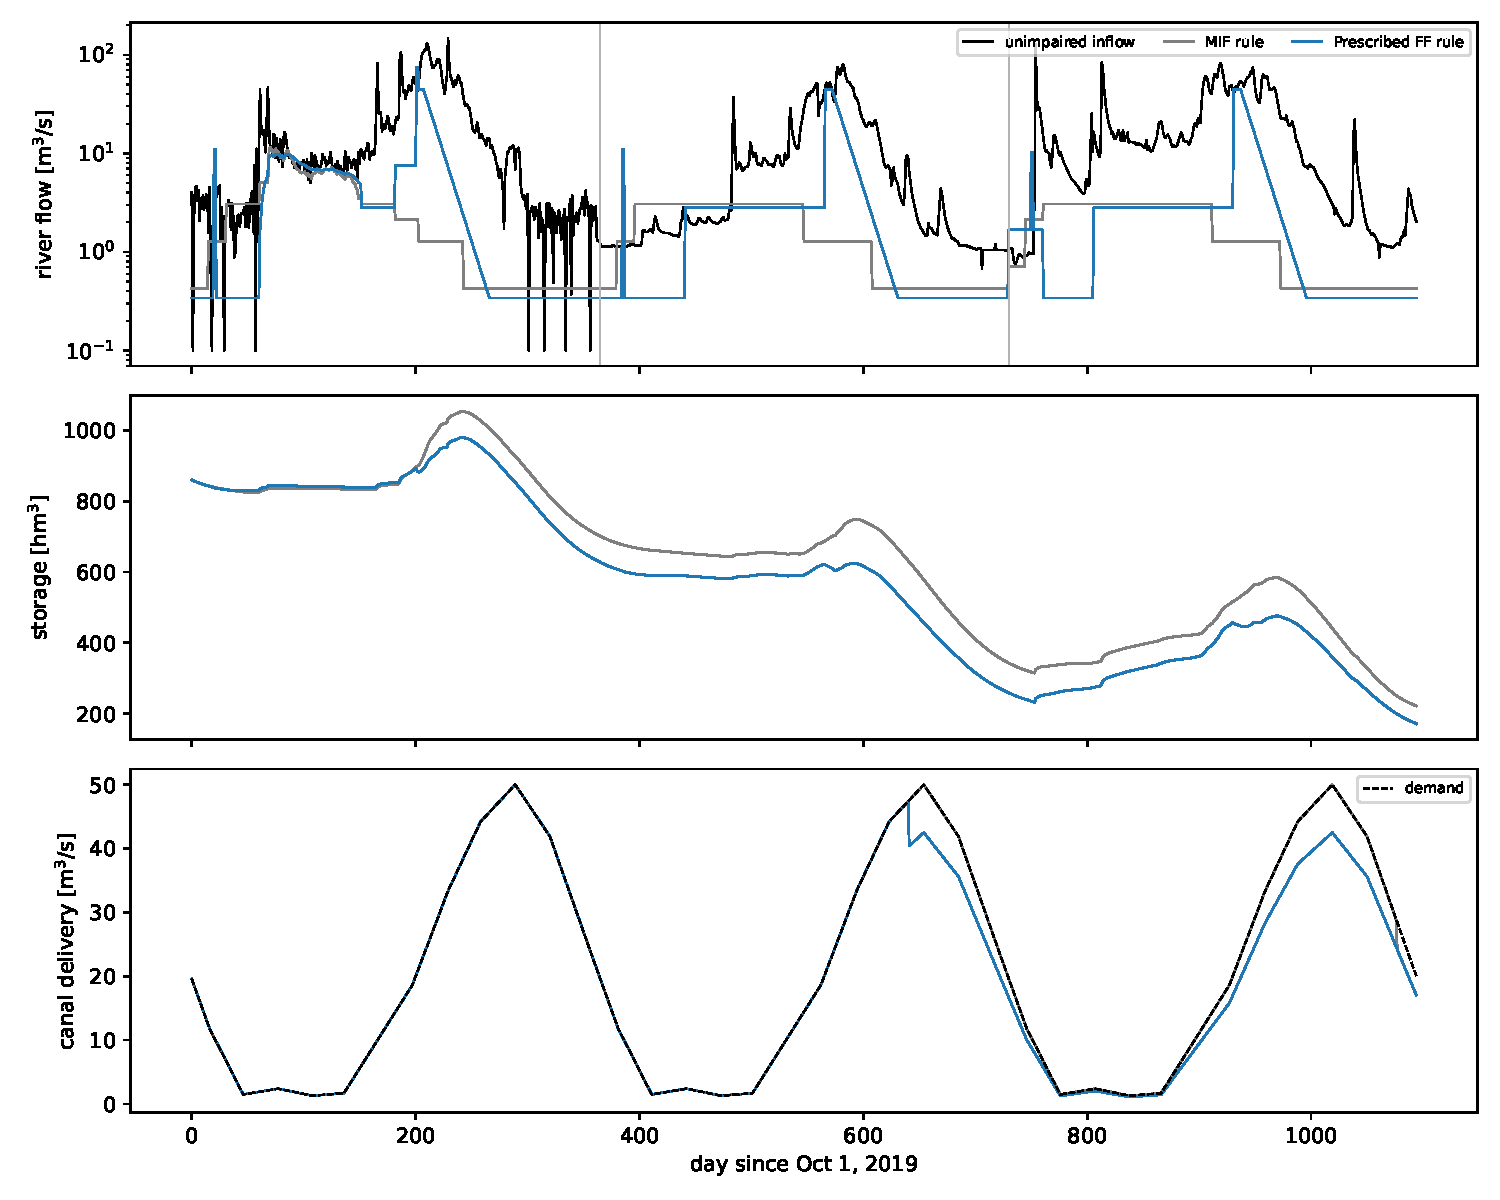
\includegraphics[width=0.92\textwidth]{figures/hydrograph_2020.pdf}
\caption{WY2020--2022, the drought. The prescription releases a spring
pulse each year (top), and storage ends each year lower than under minimum
flows (middle). In the third year this forces hedged canal deliveries
(bottom): the irrigation cost of a static e-flow schedule in a multi-year
drought.}
\label{fig:hydro2020}
\end{figure}

\begin{figure}[p]
\centering
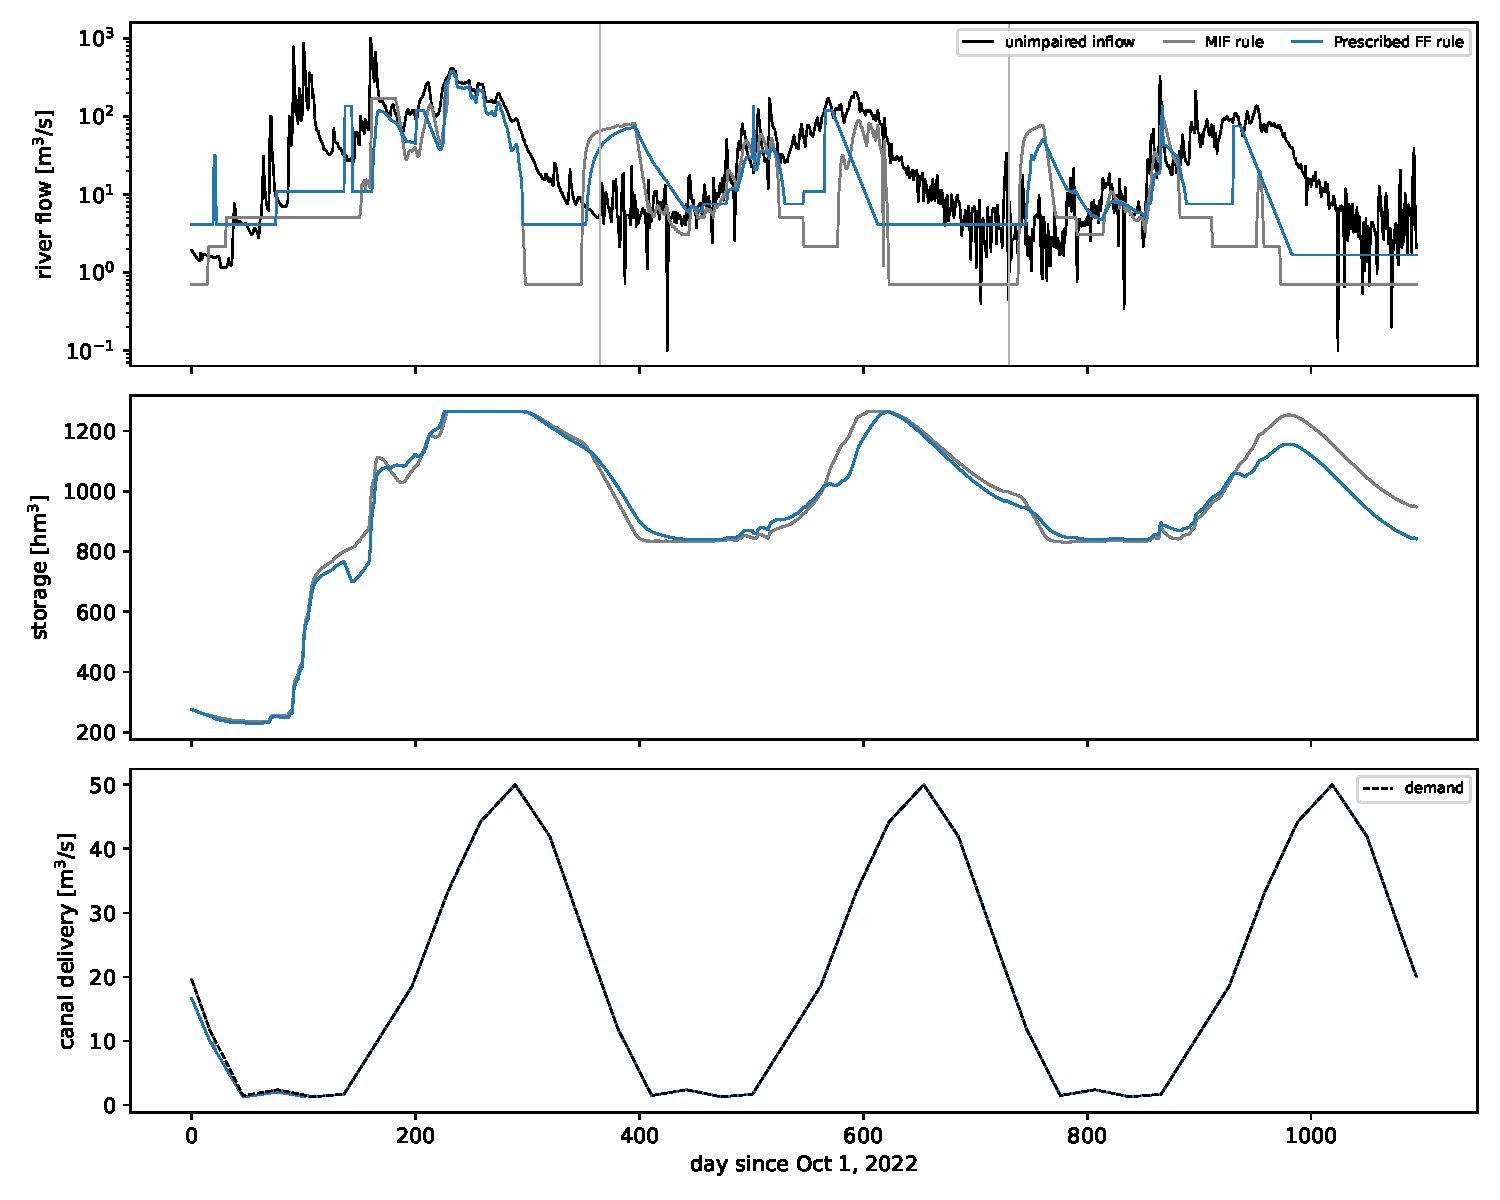
\includegraphics[width=0.92\textwidth]{figures/hydrograph_2023.pdf}
\caption{WY2023--2025 (wet, wet, moderate). After the 2020--22 drought the
reservoir starts low, and the record 2023 runoff refills it within one
season.}
\label{fig:hydro2023}
\end{figure}

\subsection{A check against observed operations}
The model is stylized, so it is worth asking whether its minimum-flow
operation looks anything like the real river. Table~\ref{tab:hist} compares,
for the years with a river record below the diversions (USGS near
Snelling, WY1989--2009), the observed river volume and functional-flow
score with those of the simulated minimum-flow rule. The observed river
scores 0.53 on average and the simulated one 0.42. In dry and wet years
the two agree closely (e.g.\ 1990, 1992, 1994, 2006, 2007). The gap is in
moderate years. There the real river carried two to four times the
licence minimum (e.g.\ 240--280~hm$^3$ against 70--150~hm$^3$ in
2002--2004) and scored 0.5--0.6 instead of 0.1--0.2. The extra water came
from operational releases that the stylized model does not represent. The
simulated minimum-flow rule is therefore a pessimistic stand-in for the
status quo in moderate years, and a close one otherwise.

\begin{table}[h]
\centering\small
\begin{tabular}{@{}llrrrr@{}}
\toprule
 & & \multicolumn{2}{c}{River volume [hm$^3$]} & \multicolumn{2}{c}{FF score}\\
\cmidrule(lr){3-4}\cmidrule(lr){5-6}
WY & type & observed & MIF rule & observed & MIF rule\\
\midrule
1989 & moderate & 123 & 72 & 0.18 & 0.10 \\
1990 & dry & 110 & 53 & 0.58 & 0.62 \\
1991 & moderate & 91 & 63 & 0.16 & 0.62 \\
1992 & dry & 128 & 56 & 0.62 & 0.62 \\
1993 & wet & 447 & 172 & 0.35 & 0.12 \\
1994 & dry & 266 & 254 & 0.87 & 0.87 \\
1995 & wet & 1343 & 1718 & 0.56 & 0.63 \\
2002 & moderate & 276 & 67 & 0.61 & 0.10 \\
2003 & moderate & 238 & 150 & 0.53 & 0.18 \\
2004 & moderate & 237 & 72 & 0.62 & 0.10 \\
2005 & wet & 943 & 826 & 0.50 & 0.27 \\
2006 & wet & 1548 & 1474 & 0.79 & 0.80 \\
2007 & dry & 330 & 119 & 0.87 & 0.87 \\
2008 & moderate & 123 & 66 & 0.30 & 0.10 \\
2009 & moderate & 177 & 78 & 0.49 & 0.10 \\

\bottomrule
\end{tabular}
\caption{Observed river flow near Snelling vs the simulated minimum-flow
operation (years with a complete record).}
\label{tab:hist}
\end{table}

\subsection{Reinforcement learning (Scenarios 3 and 4)}
\IfFileExists{results_ppo.tex}{\textbf{Result: in this set-up PPO did not improve on the tuned prescriptive
rule.} Starting from the rule exactly (residual policy, zero correction),
every PPO update made the noise-free policy \emph{worse} on the
training-period validation windows (Figure~\ref{fig:training}, right).
Checkpoint selection therefore returns update~0, i.e.\ the rule itself, and
the ``PPO'' operation on the test period is identical to the prescribed
functional-flow rule. It is not drawn separately in the figures above.
Scenario~4 (adding hydropower) was not run, since Scenario~3 gave no
learned policy to extend.

\begin{figure}[h]
\centering
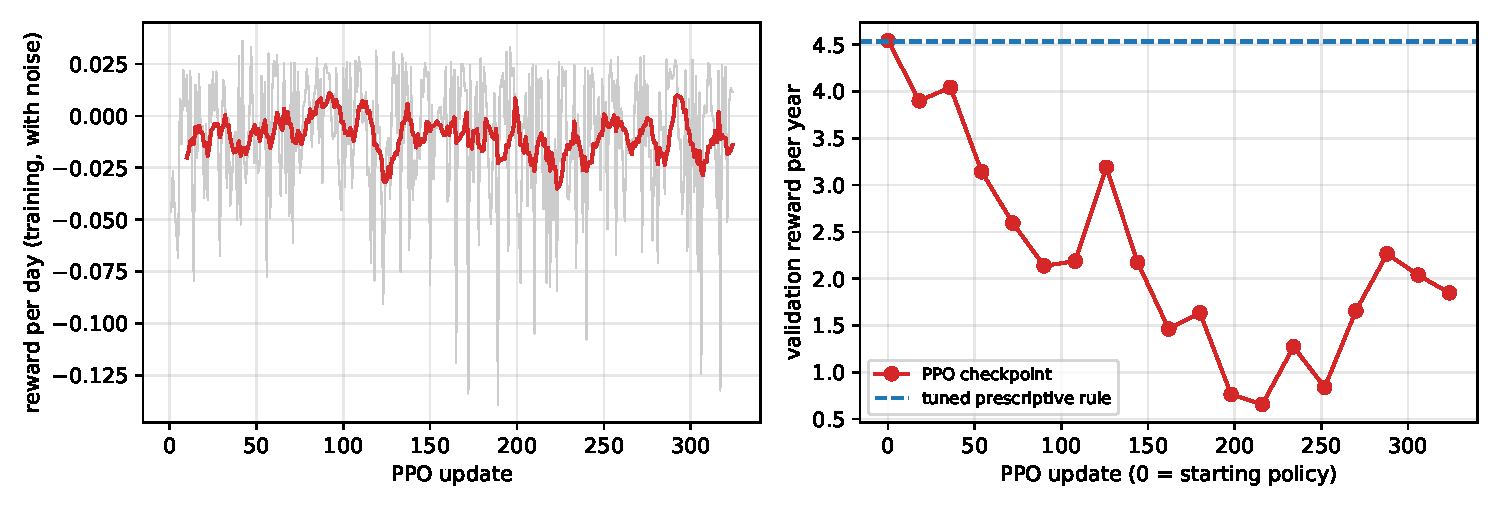
\includegraphics[width=\textwidth]{figures/training_ffreward.pdf}
\caption{Scenario~3 training. Left: mean reward per simulated day of the
noisy training policy (gray: per update; red: 10-update mean). Right: mean
reward per year of each saved checkpoint, run without noise on the five
training-period validation windows, against the tuned prescriptive rule
(dashed). Update 0 is the rule with zero correction.}
\label{fig:training}
\end{figure}

What PPO changed is clear from the reward components
(Table~\ref{tab:ppo_decomp}). The functional-flow part stayed the same
(score 0.85--0.86 throughout), but the policy released progressively more
river water: up to 19~hm$^3$/yr more than the rule. That water was missing
from irrigation in dry years, and the supply term fell from $-4.5$ to
$-7.8$ per year. In other words, the agent paid irrigation water for no
ecological gain.

\begin{table}[h]
\centering\small
\begin{tabular}{@{}lrrrrrrr@{}}
\toprule
 & reward/yr & supply & flood & FF reward & FF score & irrigation [\%] & river [hm$^3$/yr]\\
\midrule
tuned rule & 4.53 & -4.47 & -0.37 & 9.38 & 0.846 & 95.6 & 395 \\
PPO update 72 & 2.59 & -6.32 & -0.43 & 9.35 & 0.858 & 95.1 & 406 \\
PPO update 144 & 2.18 & -6.51 & -0.66 & 9.34 & 0.857 & 95.1 & 407 \\
PPO update 216 & 0.66 & -7.85 & -0.82 & 9.33 & 0.856 & 94.9 & 414 \\
PPO update 324 & 1.85 & -6.66 & -0.74 & 9.25 & 0.853 & 95.1 & 409 \\

\bottomrule
\end{tabular}
\caption{Validation windows (training period): reward components per year
for the rule and for PPO checkpoints.}
\label{tab:ppo_decomp}
\end{table}

\paragraph{Why.} The most likely explanation is a bias that Gaussian
exploration builds into this problem. During training every release
carries random noise (here $\pm4\%$). Near a target, a little extra release
protects the \emph{noisy} policy against falling short. The benefit is
immediate, on the same day, and easy to attribute. The cost (less water
in storage) appears months later, as a hedged irrigation delivery in late
summer or in the next dry year. With $\gamma=0.995$ and three-year
episodes this delayed cost is real in the return, but it is hidden under
much larger random variation between hydrologic years. PPO's advantage
estimates pick up the immediate, noise-protecting benefit and largely miss
the delayed cost. So the policy drifts toward over-releasing, which is the
right reaction for the noisy policy and the wrong one for the deployed,
noise-free policy. The training curve (left panel) shows no clear upward
trend either. The signal that would distinguish a better adaptive rule
from the prescription is small compared with the year-to-year noise.

\paragraph{What the attempts taught.} The path to this result went through
several failures, each instructive (Sections~\ref{sec:reward}
and~\ref{sec:training}):
\begin{enumerate}\itemsep2pt
\item A cloned copy of a calendar-based rule is not the rule. Small action
  errors break day-specific targets, so we learned a correction to the
  rule (residual policy) instead.
\item RL found two reward loopholes within minutes of training: near-miss
  pulse credit that could be collected indefinitely, and double payment
  when the year type changed. Every reward term needs an explicit bound.
\item A reward that differs from the evaluation score gets optimized
  instead of the score. A squared baseflow penalty let PPO shave
  baseflows. The final reward is the daily increment of the score.
\item Pass/fail ecological thresholds on daily flows, and recession limits
  on raw daily changes, make the reward hypersensitive to the exploration
  noise that policy-gradient methods rely on.
\end{enumerate}
}{The PPO agent for
Scenario~3 is being retrained with the final reward formulation
(Section~\ref{sec:training}). Its results will be added to
Table~\ref{tab:test} and Figures~\ref{fig:tradeoff}--\ref{fig:hydro2023}
when the run completes.}
